\documentclass[10pt,a4paper,twocolumn,twoside]{article}
\usepackage[utf8]{inputenc}
\usepackage[T1]{fontenc}
\usepackage[english]{babel}
\usepackage{multicol}
\usepackage{graphicx}
\usepackage{fancyhdr}
\usepackage{times}
\usepackage{titlesec}
\usepackage{multirow}
\usepackage{lettrine}
\usepackage[backend=biber, style=numeric, sorting=none]{biblatex}
\usepackage[top=2cm, bottom=1.5cm, left=2cm, right=2cm]{geometry}
\usepackage{url}
\usepackage{float}
\usepackage[figurename=Fig.,tablename=TABLE]{caption}
\usepackage{booktabs}
\usepackage{subcaption}
\usepackage{amsmath}
\usepackage{amssymb}
\usepackage{xcolor}
\usepackage{colortbl}
% \usepackage{parskip}
\addbibresource{references.bib}
\captionsetup[table]{textfont=sc}
\usepackage[hidelinks]{hyperref}
\usepackage{tikz}
\usetikzlibrary{arrows.meta,positioning,calc}

\author{\LARGE\sffamily David Morillo Massagué}
\title{\Huge{\sffamily Metastasis Prediction in Colorectal\\
Cancer with Whole Slide Images\\
using Graph Attention Networks}}

\date{}

\newcommand\blfootnote[1]{%
  \begingroup
  \renewcommand\thefootnote{}\footnote{#1}%
  \addtocounter{footnote}{-1}%
  \endgroup
}

\titleformat{\section}
{\large\sffamily\scshape\bfseries}
{\textbf{\thesection}}{1em}{}

\begin{document}

\fancyhead[LO]{\scriptsize David Morillo Massagué: Metastasis Prediction in Histopathology using GATs}
\fancyhead[RO]{\thepage} \fancyhead[LE]{\thepage}
\fancyhead[RE]{\scriptsize EE/UAB Data Engineering BSc Thesis: Metastasis Prediction in Histopathology using GATs}

\fancyfoot[CO,CE]{}

\fancypagestyle{primerapagina}
{
   \fancyhf{}
   \fancyhead[L]{\scriptsize BSC THESIS IN DATA ENGINEERING, SCHOOL OF ENGINEERING (EE), UNIVERSITAT AUTÒNOMA DE BARCELONA (UAB)}
   \fancyfoot[C]{\scriptsize June 2026, School of Engineering (UAB)}
}

\renewcommand{\headrulewidth}{0pt}
\renewcommand{\footrulewidth}{0pt}
\pagestyle{fancy}

\twocolumn[\begin{@twocolumnfalse}

\maketitle

\thispagestyle{primerapagina}

\begin{center}
\parbox{0.915\textwidth}
{\sffamily
\textbf{Abstract--}
We present an N0/N1 classification system for lymph node metastasis prediction in pT1 colorectal
cancer from Whole Slide Images. Tissue is represented as a spatial graph over patch coordinates,
preserving the real spatial topology of the tissue.
Each node is a 2048$\times$2048 px patch represented by a
CLS embedding of shape $[1, 1536]$ from the UNI2 model. Two configurable architectures are compared: a
GAT baseline with flat readout (mean, max, mean\_max or attention) and a GAT+DiffPool model
with hierarchical DiffPool interleaved between GAT layers for
multi-scale representations. Patient-level diagnosis is obtained via MIL aggregation over
histological sections. Hyperparameter search combines two Optuna studies
(5-fold CV + 90/10 retraining of the best configurations).
The best model is the GAT baseline, achieving test
AUC $=0.875$, sensitivity $100\%$ and specificity $57.5\%$.
\\
\\
\textbf{Keywords-- } pT1 colorectal cancer, Lymph node metastasis, Digital histopathology,
Graph Attention Networks, Hierarchical DiffPool, Spatial Delaunay graph, Multiple Instance Learning.\\
}

\bigskip

{\vrule depth 0pt height 0.5pt width 4cm\hspace{7.5pt}%
\raisebox{-3.5pt}{\fontfamily{pzd}\fontencoding{U}\fontseries{m}\fontshape{n}\fontsize{11}{12}\selectfont\char70}%
\hspace{7.5pt}\vrule depth 0pt height 0.5pt width 4cm\relax}

\end{center}

\bigskip
\end{@twocolumnfalse}]

\blfootnote{$\bullet$ Contact e-mail: David.MorilloMa@autonoma.cat}
\blfootnote{$\bullet$ Supervised by: Debora Gil Resina (DCC)} \blfootnote{$\bullet$ Academic year 2025/26}

\section{Introduction}

\lettrine[lines=3]{C}{olorectal} cancer (CRC) is one of the most serious public health challenges in our
setting. In Spain, the SEOM projects around 44,132 new diagnoses for 2026, making it the
most frequent tumor and the second leading cause of cancer death, with 14,629 deaths \cite{seom2026}.

pT1 carcinoma is particularly complex: the tumor has invaded the submucosa but not the muscularis propria, and the risk of
lymph node metastasis (LNM) ranges between
$2\%$ and $23\%$ depending on the depth
of invasion \cite{ParcSalutMar2013}.
When poor-prognosis criteria are present (submucosal invasion $\geq\!1000\,\mu$m,
vascular or lymphatic invasion, undifferentiated histology, \textit{tumor budding} of
grade~$\geq\!2$, or a positive vertical margin \cite{jsccr2019,dawson2024budding}), the risk rises
to around $10\%$, leading clinical guidelines (JSCCR \cite{jsccr2019}, NCCN, and
ESMO) to recommend additional radical surgery. Since most pT1
tumors do not develop real LNM, it is estimated that up to $80\%$ of these surgeries are
unnecessary \cite{zaffalon2023,MartinezDeJuan2024}.

Digital histopathology emerged in the late 1990s with the first whole-slide
scanners, and since the mid-2010s deep learning models have been applied to it to assist the pathologist \cite{bejnordi2017camelyon}. This work,
developed at the CVC~\cite{cvc} under the supervision of Dr.\ Debora Gil, addresses the
N0/N1 classification task from \textit{Whole Slide Images} (WSI) by modeling each tissue
section as a spatial graph. A GAT baseline with flat
\textit{readout} is compared against a model with hierarchical \textit{pooling} (DiffPool) interleaved between layers, and
different MIL (\textit{Multiple Instance Learning}) aggregation strategies are proposed
for patient-level diagnosis.

Two reasons motivate this work. From a clinical standpoint, AI systems can
consistently detect subtle patterns (often outperforming clinical guidelines) and help reduce unnecessary
surgeries. From a technical standpoint, combining graph attention networks with
deep learning on real-world data sits at the intersection of graph theory and deep learning
that I want to explore within Data Engineering.

\section{State of the Art}

\subsection{Clinical Guidelines and Predictive Models for pT1 CRC}
\label{sec:guidelines-sota}

The reference clinical guidelines (JSCCR \cite{jsccr2019}, NCCN, and
ESMO) recommend additional surgery when the patient
presents one or more of the histopathological risk criteria mentioned in the
Introduction. Despite their high sensitivity, their specificity
is low: in a comparative study of $560$ patients
\cite{tanino2024comparative}, the reported AUCs are $0.596$ (JSCCR),
$0.749$ (NCCN), and $0.743$ (ESMO)\footnote{Since these are binary classifiers, a guideline's AUC
equals $(\text{sens}+\text{spec})/2$ (\textit{balanced accuracy}).},
with specificities of $19\%$ (JSCCR), $52\%$ (NCCN), and $50\%$ (ESMO):
following JSCCR, more than $80\%$ of operated patients did not have real
LNM \cite{tanino2024comparative,zaffalon2023}.

In parallel, Piao et al.~\cite{piao2023ai} proposed an AI
model over clinicopathological variables ($n\!=\!546$ training,
$n\!=\!105$ test) based on gradient boosting (\textit{LightGBM}),
achieving $100\%$ sensitivity, $85.8\%$ specificity, an AUC of
$0.960$, and $92.9\%$ \textit{balanced accuracy}; the rate of
patients classified as high risk dropped from $83.8\%$ (JSCCR)
to $20.9\%$. Dawson et al.~\cite{dawson2024budding} proposed
the IBC Score, a weighted score over lymphovascular invasion, \textit{tumor budding}
grade, invasion depth, and tumor grade,
achieving an AUC of $0.68$ over $565$ patients. Unlike these
works, this thesis performs the prediction exclusively from the
histopathological image (WSI), without structured clinical variables
or manual pathologist scoring.

\subsection{WSI Classification with MIL}

\textit{Whole Slide Images} have resolutions of up to $150,000 \times 150,000$
pixels and cannot be processed directly with conventional networks. The usual approach
is to divide the slide into small \textit{patches} and work with MIL, where the model must
infer the global label (N0/N1) from fragments without
individual labels. Ilse et al.~\cite{ilse2018attentionbaseddeepmultipleinstance}
proposed attention-based aggregation (\textit{attention-based MIL}), which learns which
\textit{patches} are most relevant for diagnosis. Lu et al.~\cite{lu2020dataefficientweaklysupervised}
applied this method (CLAM) to lymph node metastasis detection in the CAMELYON challenge
(breast cancer, AUC $\sim\!0.95$); that task, however, detects metastasis \emph{present}
in the lymph node's own slide, whereas here the nodal status is predicted from the
primary tumor, so the results are not directly comparable. Li et
al.~\cite{li2021dualstreammultipleinstancelearning} proposed DSMIL, which combines two
branches, at the \textit{patch} and slide level, with contrastive learning. The
prediction of lymph node metastasis from histopathology has been studied in other cancers:
Muti et al.~\cite{muti2023deep} show that it is possible to predict N0/N1 status from
gastric cancer slides, with promising results.

\subsection{Graphs and GNNs in Digital Pathology}

Graph neural networks (GNN) make it possible
to treat tissue as a structure where
regions are connected according to their proximity, capturing spatial relations that
convolutional neural networks (CNN) do not directly model. Jaume et al.~\cite{jaume2021histocartographytoolkitgraphanalytics}
presented HistoCartography, a framework for graph analysis in digital
pathology, with results showing improvements over CNNs in biopsy
classification. This framework distinguishes between \textit{cell-graphs} (nodes = individual
cells) and \textit{tissue-graphs} (nodes = tissue regions); this work is closer
to the second type, with nodes representing tissue \textit{patches} rather than cells.
Regarding architecture, HistoCartography classifies these graphs with GIN
(\textit{Graph Isomorphism Networks}) networks, whereas this work opts for
GAT~\cite{veličković2018graphattentionnetworks}, which add an attention mechanism that
lets the model weight each neighbor differently, particularly useful in
histopathology where not all tissue regions carry the same information. Regarding
graph \textit{pooling}, Grattarola et al.~\cite{Grattarola_2024} review the
main existing methods, including DiffPool~\cite{ying2019hierarchicalgraphrepresentationlearning},
which groups nodes into super-nodes progressively.

A key decision in building these graphs is the edge criterion: some
works base them on \textit{feature similarity} between \textit{patches},
while others opt for spatial proximity between tissue regions.
This work follows the second approach and connects \textit{patches} via a
triangulation over the tissue coordinates, so that nodes and edges
preserve the real topology rather than purely semantic relations.

\subsection{Foundation Models for Histopathology}

In recent years, \textit{foundation models} pretrained specifically
on pathology data have emerged, generating embeddings far more informative than
generic CNNs. UNI2~\cite{chen2024uni2} is a \textit{vision transformer} (ViT) trained on
more than 100 million \textit{patches} from 20 tissue types, with good results across
numerous histopathological classification tasks. CONCH~\cite{lu2024conch} is a
similar model that additionally incorporates image-text alignment. This project uses
UNI2 embeddings as the feature vector for each node, since they are
pretrained in the same domain and capture relevant morphological information.

\subsection{Prior Work at the CVC on pT1 CRC}

Martí~\cite{ddd.uab.cat:317556} compared CNNs, ViTs, and GNNs on the same
pT1 CRC dataset to classify individual \textit{patches} by percentage of tumor
infiltration, obtaining the best AUC ($0.954 \pm 0.077$) with a hybrid ViT+NN
architecture. That task, however, is tissue classification at the \textit{patch}
level, without spatial topology or patient-level diagnosis, and does not predict nodal status; this thesis
builds on UNI2 CLS embeddings to construct spatial graphs of the sections
and predict N0/N1 status from a patient-level MIL perspective.

\section{Objectives}

The general objective of this work is to \textbf{classify N0/N1 nodal status} in
pT1 colorectal cancer from real WSIs, using the UNI2 model's CLS embeddings
and representing each tissue section as a spatial graph (Delaunay triangulation
over the tissue coordinates).

From this general objective the following specific objectives are derived:
\begin{itemize}
    \item Build a complete \textit{pipeline}, from generating spatial graphs
    from CLS embeddings to training and evaluating the model.
    \item Compare a GAT baseline with flat \textit{readout} against a model with
    hierarchical DiffPool interleaved between GAT layers, assessing whether progressive
    graph reduction improves intra-section representation.
    \item Implement and compare patient-level MIL aggregation strategies to integrate
    predictions from multiple histological sections.
\end{itemize}

\section{Data and Preprocessing}

This project is carried out in collaboration with a UAB team that covers everything from data
preprocessing to the creation of alternative autoencoders for feature extraction, for
subsequent classification using various models.

\subsection{Input Data}

\textbf{WSI images.} The original data consist of whole-slide images (WSI) obtained with high-resolution scanners and
stained with hematoxylin-eosin, stored in MIRAX format (\textit{.mrxs}). Dimensions range between
30,000 and 150,000 pixels per side, with a significant amount of empty space or artifacts that
require prior treatment.

The effective dataset comprises 1,607 graphs (one per histological section), from
367 patients distributed unevenly between the two classes
(Table~\ref{tab:dataset}). Of a total of 606 patients in the clinical database, 236 are discarded
due to indeterminate diagnosis (NX), and of the remaining 370 with a valid diagnosis, 3 lack
generated UNI2 embeddings, leaving 367 usable patients. Samples are split into a training+validation pool (85\%) and a
fixed test set (15\%), both stratified at the patient level. Within the pool, 5-fold
cross-validation is applied for hyperparameter search (Section~\ref{sec:training-scheme}).

\begin{table*}[t]
\centering
\caption{Dataset composition (26 hospitals). Each graph corresponds to a histological section.}
\label{tab:dataset}
\small
\begin{tabular}{lrrr|rrr}
\toprule
 & \multicolumn{3}{c|}{\textbf{Patients}} & \multicolumn{3}{c}{\textbf{Graphs (sections)}} \\
\textbf{Split} & \textbf{N0} & \textbf{N1} & \textbf{Total} & \textbf{N0} & \textbf{N1} & \textbf{Total} \\
\midrule
Pool (train+val CV) & 224 &  87 & 311 & 1133 & 219 & 1352 \\
Test                &  40 &  16 &  56 &   212  &  43 &   255  \\
\midrule
Total & 264 & 103 & 367 & 1345 & 262 & 1607 \\
\bottomrule
\end{tabular}
\end{table*}

\textbf{Annotations and masks.}
\label{sec:anotacions-masques}
Dr.\ Eva Musulén, a specialist pathologist, manually performed the annotations using
\textit{Labelme} software, identifying three categories of involvement: \textit{infiltration} (abnormal tissue
invading regions it should not), \textit{dysplasia} (abnormal cells that may become
cancerous), and a \textit{combination} of both (used in cases of diagnostic doubt). From these,
color-coded segmentation masks are obtained: red (infiltration), blue (dysplasia), and light
green (combined); Figure~\ref{fig-mask} (Appendix~\ref{app:mask}) shows an example.

\subsection{Graph Construction}

\textbf{From \textit{patch} to node.} A non-overlapping sliding window is applied
to divide each slide into
$2048 \times 2048$ pixel \textit{patches} at full resolution. For each window, the
percentage of tissue in the corresponding region of the annotated binary mask is checked;
windows with no tissue pixels are discarded.
The UNI2 model~\cite{chen2024uni2} processes each \textit{patch} individually and extracts the
\textit{CLS} token from its output, obtaining a vector of shape $[1, 1536]$ that condenses the
patch's morphological and textural information. Each CLS vector becomes a graph node,
retaining the patch coordinates for edge construction.

\textbf{The section graph.}
\label{sec:model-dades}
Formally, each histological section is represented as a graph
$\mathcal{G} = (\mathbf{X},\,\mathbf{A})$, where $\mathbf{X} \in \mathbb{R}^{N \times 1536}$ is the feature
matrix of the $N$ nodes (\textit{patches}) and $\mathbf{A} \in \{0,1\}^{N \times N}$ the adjacency
matrix built via Delaunay triangulation followed by edge pruning. Each section
generates an independent graph; a patient's $S$ sections are processed separately and the
probabilities $\{P(\text{N1}_i)\}_{i=1}^{S}$ are aggregated via MIL (Section~\ref{sec:mil}). As an alternative,
a per-patient \textit{mega-graph} was explored (block-diagonal over all sections, with no edges between them), but it
gave worse results, likely because it forces a single global \textit{pooling} over physically disconnected tissues.

\textbf{Delaunay connectivity.} Patch centers form a regular grid, but connecting them with a fixed
grid is not enough: the mask leaves irregular tissue gaps and does not connect nearby regions at angles
other than 90°.
For this reason, nodes are connected via a \textbf{Delaunay triangulation} over their coordinates, which
adapts to any distribution. Edges are then pruned in two steps: those that
cross background pixels (mask with RGB value $=0$) are removed, so as not to join regions separated by empty space, as are those that
exceed twice the mean edge length, to avoid overly long connections. The result
(Figure~\ref{fig:preprocess}, with pruned edges in red) is a local mesh between
neighboring \textit{patches}.

\begin{figure*}[h]
    \centering
    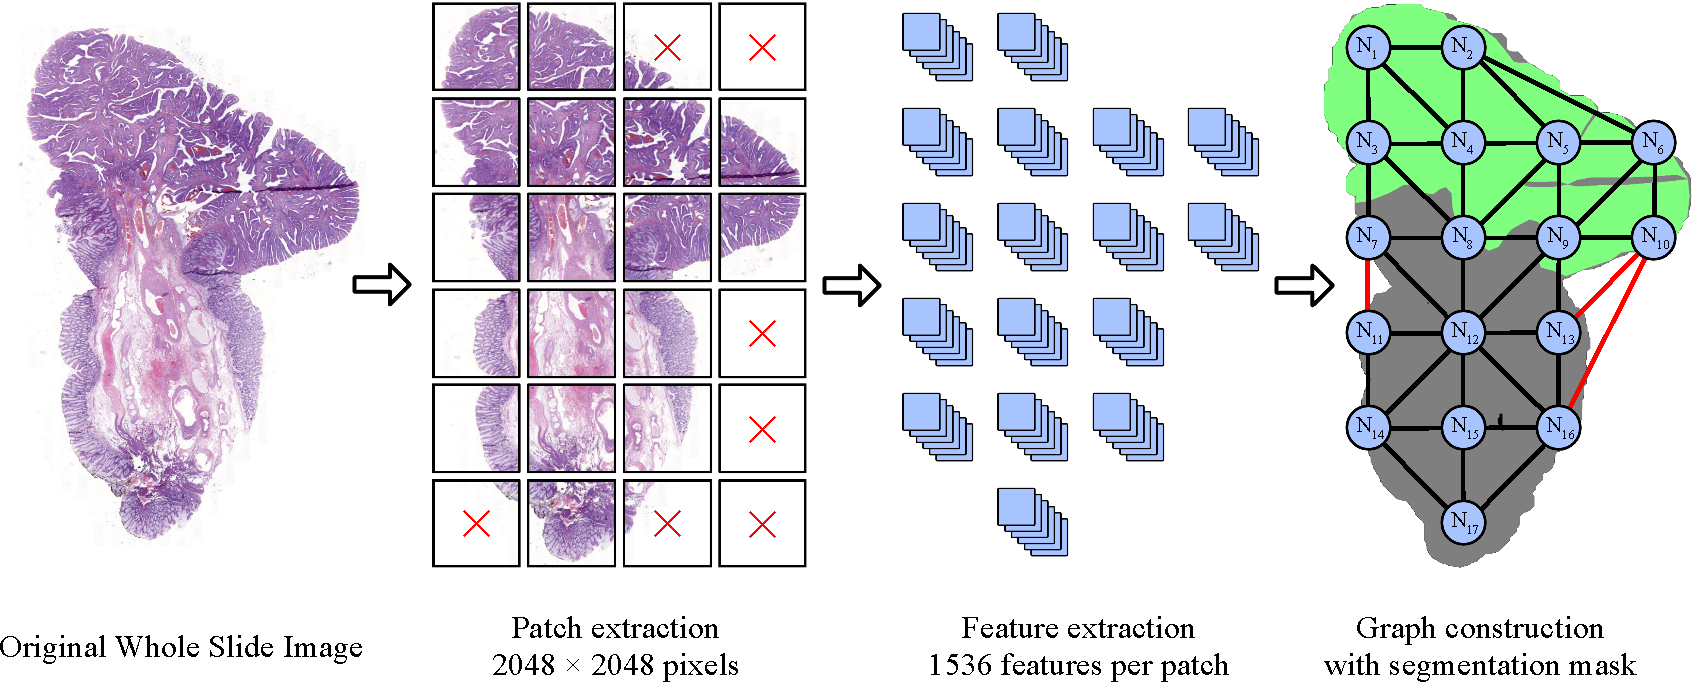
\includegraphics[width=0.9\textwidth]{img/preprocess-eng.pdf}
    \caption{Preprocessing stages for graph construction. From left to right:
    original WSI $\to$ $2048{\times}2048$ px \textit{patch} extraction via sliding window + filtering
    $\to$ CLS embedding extraction of shape $[1, 1536]$ via UNI2 (one vector per \textit{patch})
    $\to$ construction of the Delaunay graph over the annotated mask, where red edges have
    been removed by the mask filter}
    \label{fig:preprocess}
\end{figure*}

\section{Model Architecture}

\subsection{Pipeline overview}
\label{sec:pipeline-overview}

At a high level, the system can be summarized in five chained blocks
(Figure~\ref{fig:pipeline-overview}): \textbf{(1) Preprocessing}, which converts each WSI into
a spatial graph (2048$\times$2048 \textit{patch} extraction, CLS embedding $[1, 1536]$ with the
UNI2 \textit{foundation} model, and Delaunay graph construction with edge pruning);
\textbf{(2) Architecture}, where GAT layers propagate information across the graph according to one of the
two compared variants (flat \textit{baseline} or with hierarchical DiffPool);
\textbf{(3) Readout}, the final read-out that collapses the graph into a single embedding (mean, max,
mean\_max, or attention), identical for both architectures; \textbf{(4) MIL}, which
aggregates the predictions of a patient's sections (mean, max, noisy-OR, or attention); and
\textbf{(5) Decision}, where the threshold $t^*$ derived from the \textit{validation set} is applied to
obtain the binary N0/N1 classification.

\begin{figure}[h]
\centering
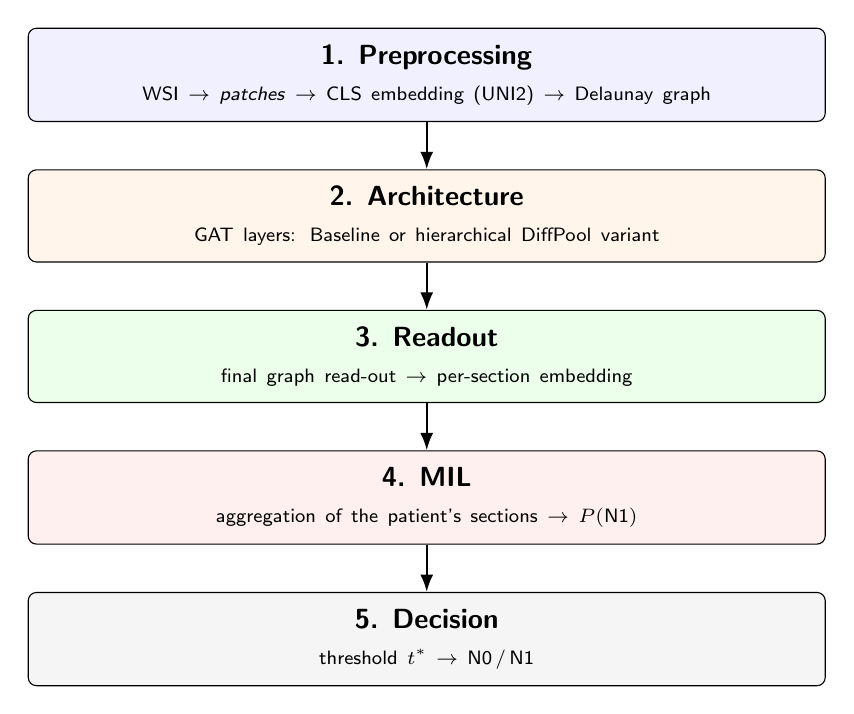
\begin{tikzpicture}[
  font=\sffamily,
  block/.style={draw, rounded corners=3pt, align=center, text width=0.80\linewidth, inner sep=6pt},
  arr/.style={-{Latex[length=2.2mm]}, thick},
  node distance=6mm
]
\node[block, fill=blue!6]  (pre)  {\textbf{1. Preprocessing}\\[1pt]\scriptsize WSI $\to$ \textit{patches} $\to$ CLS embedding (UNI2) $\to$ Delaunay graph};
\node[block, fill=orange!8, below=of pre]  (arch) {\textbf{2. Architecture}\\[1pt]\scriptsize GAT layers: Baseline or hierarchical DiffPool variant};
\node[block, fill=green!8, below=of arch]  (read) {\textbf{3. Readout}\\[1pt]\scriptsize final graph read-out $\to$ per-section embedding};
\node[block, fill=red!6, below=of read]    (mil)  {\textbf{4. MIL}\\[1pt]\scriptsize aggregation of the patient's sections $\to$ $P(\text{N1})$};
\node[block, fill=gray!8, below=of mil]    (thr)  {\textbf{5. Decision}\\[1pt]\scriptsize threshold $t^*$ $\to$ N0\,/\,N1};
\draw[arr] (pre) -- (arch);
\draw[arr] (arch) -- (read);
\draw[arr] (read) -- (mil);
\draw[arr] (mil) -- (thr);
\end{tikzpicture}
\caption{Overview of the five-block \textit{pipeline}.}
\label{fig:pipeline-overview}
\end{figure}

The following sections detail each block: the GAT architecture and its two variants, the
unified \textit{readout}, MIL aggregation, and the training procedure.

\subsection{GATClassifier}

The implemented model, \textit{GATClassifier}, is a graph classifier based on
\textbf{Graph Attention Network} layers (\textit{GATConv}~\cite{veličković2018graphattentionnetworks,fey2019fastgraphrepresentationlearning})
for binary N0/N1 classification. The architecture is fully parametrizable: the number of
GAT layers, the hidden dimension, and the number of attention heads are chosen as hyperparameters, and the
whole model is trained \textit{end-to-end} (a single backpropagation pass propagates gradients
from the final MLP head down to the first GAT layers). Building on this common base, two
architecture variants are compared, described in Section~\ref{sec:architectures}: a \textit{baseline} and one
with hierarchical DiffPool.

\textbf{Attention mechanism.} Unlike classical convolutional networks on graphs that treat
all of a node's neighbors uniformly, GAT learns to assign differentiated importance weights to each
neighbor. Given the representation $\mathbf{h}_i$ of node $i$, for each pair of neighboring
nodes $(i, j)$ an attention coefficient is computed:
\begin{equation*}
  e_{ij} = \text{LeakyReLU}\!\left(\mathbf{a}^{\top}[\mathbf{W}\mathbf{h}_i \,\|\, \mathbf{W}\mathbf{h}_j]\right)
\end{equation*}
where $\mathbf{W}$ is a learnable linear transformation, $\|$ is concatenation, and $\mathbf{a}$ a
learnable vector. The coefficients are normalized with \textit{softmax} over all neighbors:
\begin{equation*}
  \alpha_{ij} = \frac{\exp(e_{ij})}{\sum_{k \in \mathcal{N}(i)} \exp(e_{ik})}
\end{equation*}
and the new node representation is obtained as the weighted sum:
\begin{equation*}
  \mathbf{h}'_i = \sum_{j \in \mathcal{N}(i)} \alpha_{ij}\,\mathbf{W}\mathbf{h}_j
\end{equation*}

\textbf{Multi-head and non-linearity.} To increase expressive capacity, each layer uses $H$ independent
attention heads, parametrized by $\mathbf{W}^{(h)}$ and $\mathbf{a}^{(h)}$.
The outputs are concatenated at intermediate layers and averaged at the last one. The
\textit{GATConv} layer applies no final activation within the layer itself; the non-linearity is applied externally
as \textit{BatchNorm}~$\to$~ELU~$\to$~\textit{Dropout}. The only \textit{internal} non-linearity is
the \textit{LeakyReLU} in the computation of $e_{ij}$.

\subsection{The two architectures: Baseline and DiffPool}
\label{sec:architectures}

Building on the GAT layers described above, two architectures are compared that differ in
how they process the graph before the final \textit{readout}. Figure~\ref{fig-diffpool}
shows one instance of each, and Appendix~\ref{app:model-variants} presents a
detailed diagram with all configurable axes.

\textbf{GAT Baseline (flat).} Stacks $L$ consecutive GAT layers ($L$ tunable)
that always operate on the graph's original $N$ nodes, without reducing it. All
spatial information is preserved up to the final \textit{readout}.

\textbf{GAT+DiffPool (hierarchical).} Interleaves \textbf{DiffPool}
\cite{ying2019hierarchicalgraphrepresentationlearning} blocks between GAT layers. The idea is to
group nodes into \textit{super-nodes} and replace the graph with a smaller one; repeating this
several times yields a multi-scale representation of the tissue. Each block learns, for each
node, a \textit{soft assignment} to the $K$ super-nodes of the next level:
instead of sending each node to a single group, it distributes membership across all groups with weights
summing to 1 (the output of a small per-node MLP followed by \textit{softmax}). From this
assignment, node \textit{features} are aggregated as a weighted average to form those of the
super-nodes, and the original edges are projected onto the new graph, so the graph goes from $N$ to
$K \ll N$ nodes while retaining a compressed version of its structure. The number of interleaved
blocks is an optimization axis, $L_{\text{DP}}$, with one GAT layer before, between, and after
each one (total $L_{\text{DP}}+1$ GAT layers).

\textbf{DiffPool auxiliary loss.} For each block, two regularization terms are added over the
learned assignment: one that pushes neighboring nodes to be grouped together, and another (entropy-based) that makes
each node assign cleanly to few groups. The total loss is the classification
\textit{cross-entropy} plus $\lambda_{\text{aux}}$ times these terms, with $\lambda_{\text{aux}}$ as an
optimization axis.

As an alternative to DiffPool, SAGPool~\cite{lee2019selfattentiongraphpooling} selects the $K$
most relevant nodes via self-attention scores (discrete selection, not soft assignment); DiffPool was
preferred for its continuous expressiveness and the auxiliary regularization loss.

\begin{figure*}[h]
    \centering
    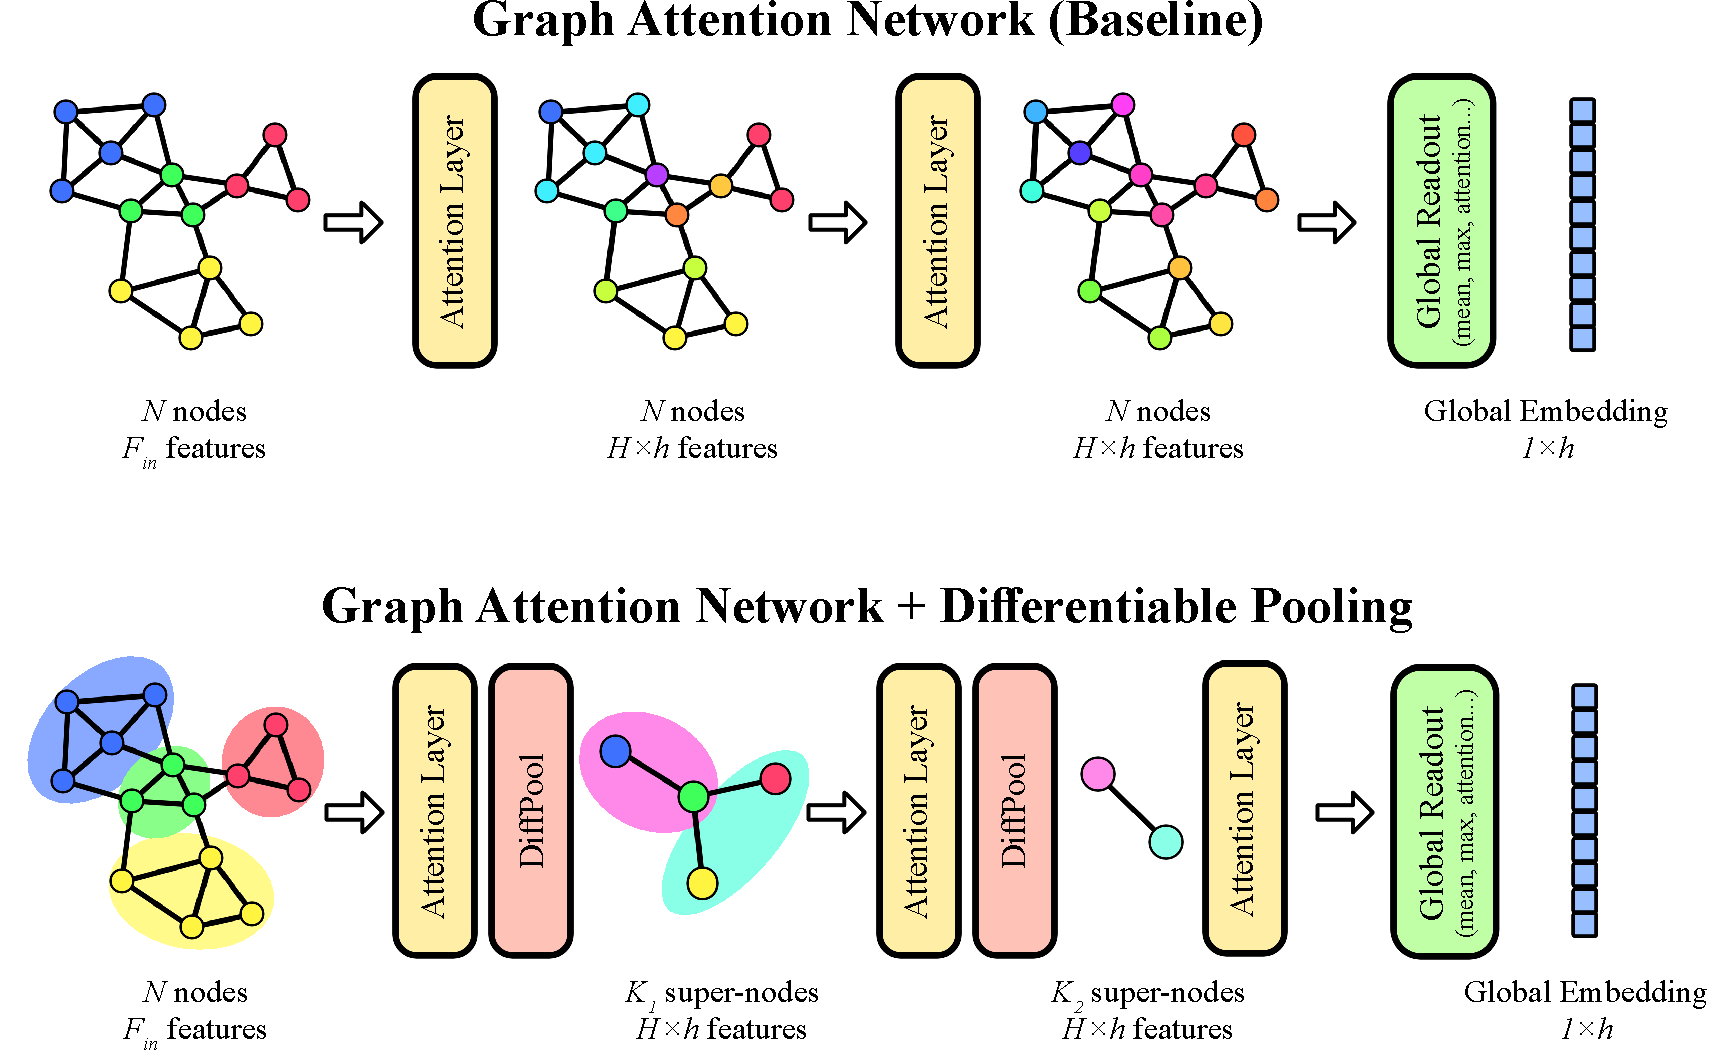
\includegraphics[width=0.9\textwidth]{img/baseline_vs_diffpool.pdf}
    \caption{Visual comparison of the two configurable architectures
    (one instance of each branch with two processing layers).
    \textbf{Top}: GAT Baseline, where two attention layers operate on the $N$
    original nodes and a global \textit{readout} produces the final embedding.
    \textbf{Bottom}: GAT+DiffPool with two DiffPool blocks ($L_{\text{DP}}=2$, i.e.\ three interleaved
    GAT layers), which progressively collapse the graph down to, in this case, two final super-nodes.}
    \label{fig-diffpool}
\end{figure*}

\subsection{Readout: final graph read-out}
\label{subsec:readout}

Whatever the architecture, the last step before classification is the same: a global
\textit{readout} that collapses the final set of nodes into a single vector
$\mathbf{h}_s$ representing the whole section. The only difference is which nodes it is applied to: in the
Baseline these are the $N$ nodes of the last GAT layer, and in DiffPool the
final $K_{L_{\text{DP}}}$ super-nodes. The \textit{readout} operation is thus an axis
shared by both branches, with four configurable options: \textit{mean}, \textit{max},
or \textit{mean\_max} (fixed aggregations), and \textit{attention}, which learns a scalar weight per node via
a linear layer followed by \textit{softmax} and aggregates via weighted sum.

Finally, the MLP head (\textit{Linear}~$\to$~ReLU~$\to$~\textit{Dropout}~$\to$~\textit{Linear})
transforms this global representation $\mathbf{h}_s$ into the section's N0/N1 logits.

\subsection{Patient-Level Aggregation (MIL)}
\label{sec:mil}

Diagnosis is per \textbf{patient}, not per slide. A given histological section may show no
visible signs of metastasis when analyzed in isolation, while another section from the same patient does
show it. If trained at the slide level, N1 sections from N1 patients that show no visible metastasis
would receive an incorrect supervision signal (N0), contaminating training.

To avoid this problem, the \textbf{Multiple Instance Learning} paradigm is used
(MIL~\cite{dietterich1997mil}): each patient is treated as a \textit{bag} and all of their
slides share the same label. The model learns to classify the patient from
their sections, without needing individual per-slide labels.

In all cases, the MLP head has the same structure:
\textit{Linear}($h$)~$\to$~ReLU~$\to$~\textit{Dropout}~$\to$~\textit{Linear}($2$), where
$h$ is the hidden dimension (hyperparameter) and the output is a pair of logits (N0/N1);
the weights are learned via backpropagation. The difference between strategies is \emph{when} it is applied:

\begin{itemize}
    \item \textbf{Mean, Max, Noisy-OR}: the MLP is applied \textbf{per section}, producing
    $P(\text{N1})_s$ for each of the patient's $S$ sections; the probabilities
    are aggregated as scalars:
    \begin{itemize}\itemsep0pt
        \item \textbf{Mean}: $P(\text{N1}_{p}) = \frac{1}{S}\sum_i p_i$.
        \item \textbf{Max}: $P(\text{N1}_{p}) = \max_i\,p_i$.
        \item \textbf{Noisy-OR}: $P(\text{N1}_{p}) = 1 - \prod_{i}(1 - p_i)$.
    \end{itemize}
    \item \textbf{Attention MIL} (\textit{gated attention},
    Ilse et al.~\cite{ilse2018attentionbaseddeepmultipleinstance}): the embeddings of the
    $S$ sections ($\mathbb{R}^{h}$ each) are first aggregated into a single patient vector
    via learned attention weights (weighted sum of the embeddings); the MLP is applied
    \textbf{only once} to this vector to obtain the N0/N1 logits. The
    internal dimension of the attention module is fixed ($128$) and is not part of the hyperparameter search.
\end{itemize}

\section{Experimental Design}

\subsection{Data and evaluation scheme}
\label{sec:training-scheme}

The dataset is split into an 85\% pool and a 15\% test set, stratified at the
patient level (Figure~\ref{fig:split-scheme}). All search (hyperparameter and
threshold selection) is done only on the pool, so the test set plays no part in any decision and provides an
unbiased performance estimate. The procedure has three stages:

\begin{enumerate}\itemsep1pt
  \item \textbf{Test (15\%, 56 patients):} separated from the moment the graphs are built and held out
        for evaluating the best models per architecture.
  \item \textbf{Bayesian search + 5-\textit{fold} CV over the pool (85\%, 311 patients):} each
        configuration is evaluated with per-patient \textit{Stratified K-Fold} and \textit{early stopping}
        (\textit{patience}$=\!20$), independently for each architecture. The search uses the
        \textit{Tree-structured Parzen Estimator} (TPE) over $\sim$15 axes: the first 200
        \textit{trials} ($\sim$10$\times$ dimensions) are random uniform sampling (exploration), and
        afterward TPE exploits the history. The maximized objective is
        $\overline{\text{spec}}_{\text{CV}} - 10\cdot\max(0, 1-\overline{\text{sens}}_{\text{CV}})$:
        mean specificity, strongly penalizing drops in sensitivity (Appendix
        \ref{app:sweep-config}).
  \item \textbf{Final retraining and test evaluation:} with the best hyperparameters for each
        architecture, the pool is split again 90/10 (internal train/val for \textit{early stopping}),
        and the final model is evaluated \textbf{once} on the test set (15\%) with the threshold $t^*$,
        the median of the 5 $t^*$ values obtained across the CV \textit{folds}.
\end{enumerate}

\begin{figure}[h]
\centering
\scalebox{0.90}{%
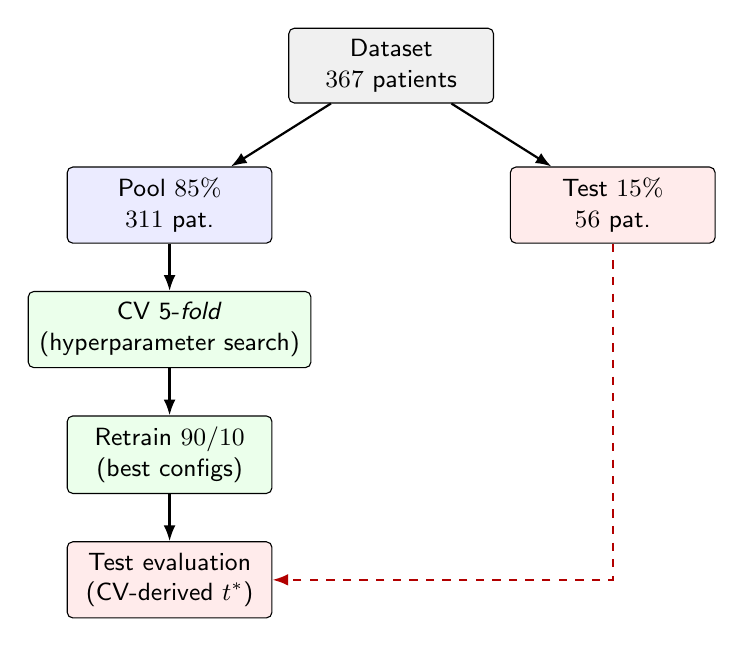
\begin{tikzpicture}[
  font=\sffamily\small,
  box/.style={draw, rounded corners=2pt, align=center, inner sep=4pt, minimum height=8mm, minimum width=2.6cm},
  proc/.style={box, fill=green!8},
  arr/.style={-{Latex[length=2mm]}, thick},
  node distance=6mm and 9mm
]
\node[box, fill=gray!12] (all) {Dataset\\$367$ patients};
\node[box, fill=blue!8, below left=8mm and 2mm of all]  (pool) {Pool $85\%$\\$311$ pat.};
\node[box, fill=red!8,  below right=8mm and 2mm of all]  (test) {Test $15\%$\\$56$ pat.};
\node[proc, below=of pool] (cv)   {CV 5-\textit{fold}\\(hyperparameter search)};
\node[proc, below=of cv]   (retr) {Retrain $90/10$\\(best configs)};
\node[box, fill=red!8, below=of retr] (eval) {Test evaluation\\(CV-derived $t^*$)};
\draw[arr] (all) -- (pool);
\draw[arr] (all) -- (test);
\draw[arr] (pool) -- (cv);
\draw[arr] (cv) -- (retr);
\draw[arr] (retr) -- (eval);
\draw[arr, dashed, red!70!black] (test) |- (eval);
\end{tikzpicture}%
}% end scalebox
\caption{Split and evaluation scheme. The test set (15\%) is isolated from the start and used only
at the end (dashed arrow).}
\label{fig:split-scheme}
\end{figure}

\subsection{Class Imbalance and Operating Threshold}

The dataset shows a strong imbalance (approximately $72\%$ N0 and $28\%$ N1). In metastasis detection, a
false negative is more serious than a false positive: the clinical goal is to maximize
specificity while keeping sensitivity $\approx$ 100\%, to reduce unnecessary surgeries
without missing any N1 case. Three complementary mechanisms are applied:
\begin{itemize}\itemsep1pt
  \item \textbf{Stratified split} by patient (keeps the N0/N1 ratio in each subset).
  \item \textbf{Cross-entropy weighting} with a positive weight $w_+$ (gradient
        multiplier for the N1 class) as an optimization axis, $w_+ \in [1.5,\,8]$.
  \item \textbf{Operating threshold derived from val} ($t^*$): two criteria were compared:
        (T1) fixed threshold $t\!=\!0.5$; and (T2) the maximum threshold on the val ROC curve that
        keeps TPR$\!=\!1$ (zero false negatives on validation). For T2, the
        threshold is computed on each \textit{fold} and its median is applied to the test set.
\end{itemize}

\subsection{Evaluation Metrics}

The main metrics are AUC-ROC (overall ranking, threshold-independent) and the
clinical metrics at the operating threshold: sensitivity ($\text{TP}/(\text{TP}+\text{FN})$),
specificity ($\text{TN}/(\text{TN}+\text{FP})$), positive predictive value
(PPV, $\text{TP}/(\text{TP}+\text{FP})$), and negative predictive value
(NPV, $\text{TN}/(\text{TN}+\text{FN})$), where TP, TN, FP, and FN are true/false positives and
negatives.

\textbf{Clinical interpretation.} If the model's output were used to decide on surgery (operating on
cases predicted as N1), sensitivity is the percentage of N1 patients who would receive
treatment (a sensitivity of $100\%$ means no patient with metastasis would go
untreated), and specificity is $1$ minus the percentage of N0 patients operated on
unnecessarily.

\subsection{Tools and Reproducibility}

The implementation follows a modular design: graph construction, the model, the training
code, and the Bayesian \textit{sweep} are decoupled, and configuration is managed via
YAML files. The search is orchestrated with \textit{Optuna}, with persistent, resumable
\textit{SQLite} \textit{storage} (no \textit{trial} is lost if the process is interrupted). To ensure
reproducibility, all \textit{sampler} draws, CV \textit{folds}, and weight
initialization use a fixed \textit{seed}. The code is available in the project's public
repository~\cite{morillo2026repo}, which includes as a submodule the model and search code,
developed jointly with other team members~\cite{morillo2026codi}.

\section{Results}

Two isolated per-architecture Optuna TPE studies were optimized, and the best
configurations of each branch (GAT Baseline and GAT+DiffPool) were re-evaluated following the
procedure in Section~\ref{sec:training-scheme} (5-fold CV + 90/10 retrain + test
evaluation). Table~\ref{tab:configs-compare} summarizes the most relevant ones.

\begin{table*}[t]
\centering
\caption{Best configurations per architecture, compared by AUC under 5-\textit{fold}
cross-validation.}
\label{tab:configs-compare}
\small
\begin{tabular}{lcccccc}
\toprule
\textbf{Architecture} & \textbf{Readout} & \textbf{MIL}
  & \textbf{$h$} & \textbf{$H$} & \textbf{dropout} & \textbf{AUC CV} \\
\midrule
\textbf{Baseline}  & \textbf{attention} & \textbf{mean} & $\mathbf{256}$ & $\mathbf{4}$ & $\mathbf{0.3}$ & $\mathbf{0.862\!\pm\!0.038}$ \\
DiffPool           & mean\_max          & mean          & $128$          & $2$          & $0.44$         & $0.847\!\pm\!0.048$ \\
\bottomrule
\end{tabular}
\end{table*}

\textbf{Reading the results.} \textbf{GAT Baseline clearly outperforms GAT+DiffPool}
on this dataset: the best DiffPool reaches a test AUC of $0.786$, $9$ points below the
Baseline ($0.875$). Sections have only a few hundred \textit{patches}, and
hierarchical reduction to super-nodes discards more information than it synthesizes. Moreover,
only the Baseline maintains sens.\ $=100\%$ on the test set with the $t^*$ threshold derived from val.

\textbf{Selected model.} The final model is a GAT Baseline with \textit{attention}
\textit{readout}, \textit{mean} MIL, $h=256$, $H=4$, \textit{dropout} $0.3$,
$\lambda_{\text{wd}}=10^{-4}$, $\eta=3\!\cdot\!10^{-4}$, and Adam with \textit{ReduceLROnPlateau}.
It achieves AUC CV $0.862\pm 0.038$, test AUC $0.875$, sensitivity $100\%$ (16/16 N1), and
specificity $57.5\%$ at threshold $t^*\!=\!0.133$.

\subsection{Hyperparameter Importance}
\label{sec:main-effects}

The \textit{fANOVA} importance analysis for each study (full table in
Appendix~\ref{app:main-effects}) shows that MIL aggregation is the most
determinant axis of performance for the Baseline ($I=0.64$; no other axis exceeds $10\%$),
while for DiffPool the importance is spread between MIL ($0.22$), the auxiliary
weight $\lambda_{\text{aux}}$ ($0.14$), and the \textit{learning rate} ($0.13$).

\subsection{Comparison with Clinical Guidelines and SOTA}
\label{sec:resultats-comparacio}

Table~\ref{tab:comparison} positions the selected model against the reference clinical
guidelines (Section~\ref{sec:guidelines-sota}) and two AI models (one over
clinical variables and another over WSI images).
The guideline figures come from~\cite{tanino2024comparative} ($n\!=\!560$),
while the GAT figures were obtained on this work's test set ($n\!=\!56$;
N1 prevalence $28.6\%$, higher than the real clinical rate of $\sim\!8$–$15\%$
\cite{zaffalon2023}). Sensitivity and specificity are independent of
prevalence and form the basis of the comparison; PPV must be interpreted with
caution (Section~\ref{sec:limitacions}).

\begin{table*}[h]
\centering
\caption{Performance comparison between the proposed model, clinical guidelines, and the state of the art.
Each system comes from an independent study and population
(Tanino $n\!=\!560$; IBC Score $n\!=\!565$; LightGBM $n\!=\!105$; Song $n\!=\!1281$; GAT $n\!=\!56$),
so PPV is not directly comparable. Bal.Acc.~$=(S\!+\!E)/2$.}
\label{tab:comparison}
\small
\begin{tabular}{llrrrr}
\toprule
\textbf{System} & \textbf{Input type} & \textbf{Sensitivity} & \textbf{Specificity} & \textbf{AUC} & \textbf{Bal.Acc.} \\
\midrule
\multicolumn{6}{l}{\textit{Guidelines and clinical scores}} \\[2pt]
JSCCR \cite{jsccr2019}        & Clinical guideline  & $100\%$ & $19\%$  & $0.596$ & $59.5\%$ \\
NCCN                           & Clinical guideline  & $98\%$  & $52\%$  & $0.749$ & $75.0\%$ \\
ESMO \cite{tanino2024comparative} & Clinical guideline  & $98\%$  & $50\%$  & $0.743$ & $74.0\%$ \\
IBC Score \cite{dawson2024budding} & Histopath.\ score & $90\%$ & $26\%$ & $0.68$ & $58.0\%$ \\
\midrule
\multicolumn{6}{l}{\textit{AI models}} \\[2pt]
LightGBM \cite{piao2023ai}                          & Clinicopathol.\ var. & $100\%$  & $85.8\%$ & $0.960$ & $92.9\%$ \\
Song et al.\ \cite{song2024lnm}                     & WSI image & $92.9\%$ & $57.6\%$ & $0.781$ & $75.3\%$ \\
\multicolumn{6}{l}{\textit{GAT Baseline (AUC $= 0.875$)}} \\[1pt]
\quad T1 ($t\!=\!0.5$)                                        & WSI image & $56.2\%$ & $92.5\%$ & $0.875$ & $74.4\%$ \\
\textbf{\quad T2 ($t^*\!=\!0.133$, TPR$=1$)$^{\dagger}$}     & \textbf{WSI image} & $\mathbf{100\%}$ & $\mathbf{57.5\%}$ & $\mathbf{0.875}$ & $\mathbf{78.8\%}$ \\[2pt]
\multicolumn{6}{l}{\textit{GAT+DiffPool (AUC $= 0.786$)}} \\[1pt]
\quad T1 ($t\!=\!0.5$)                                        & WSI image & $50.0\%$ & $82.5\%$ & $0.786$ & $66.3\%$ \\
\quad T2 ($t^*\!=\!0.303$)$^{\dagger}$                       & WSI image & $62.5\%$ & $70.0\%$ & $0.786$ & $66.3\%$ \\
\bottomrule
\end{tabular}\\[2pt]
\footnotesize{$^{\dagger}$\,$t^*$ is the median of the maximum TPR$=1$ thresholds across the 5 \textit{val sets}, applied to the test set without readjustment.}
\end{table*}

Since a false negative (failing to treat an N1 case) is clinically unacceptable, \textbf{T2 is the only
acceptable option}: T1 ($t\!=\!0.5$) leaves $7$ of $16$ N1 patients undetected (\textbf{FN$=7$}),
while T2 ($t^*\!=\!0.133$, TPR$=1$) guarantees zero false negatives
(\textbf{sens.$=100\%$}, \textbf{NPV$=1.000$}). The resulting specificity ($57.5\%$) exceeds
the JSCCR guideline ($19\%$) and the IBC Score ($26\%$), and is comparable to NCCN ($52\%$) and ESMO ($50\%$).
Figure~\ref{fig:cv-roc} shows the ROC curves of the CV's 5 \textit{val sets} and the
individual operating points; the median of the 5 thresholds is $t^*\!=\!0.133$.
Figure~\ref{fig:roc-top5} overlays the test ROC curves with the clinical guidelines.

\begin{figure}[h]
\centering
\includegraphics[width=0.48\textwidth]{img/cv_roc-eng.pdf}
\caption{ROC curves of the 5 cross-validation \textit{folds} (GAT Baseline). Each circle
marks the maximum TPR$=1$ threshold of its \textit{fold}; the median of the 5 thresholds
($t^*\!=\!0.133$, yellow box) is applied to the test set.}
\label{fig:cv-roc}
\end{figure}

\begin{figure}[h]
\centering
\includegraphics[width=0.48\textwidth]{img/roc_top5-eng.pdf}
\caption{ROC curves on the test set ($n\!=\!56$) for the GAT Baseline (selected model;
AUC $=0.875$) and GAT+DiffPool (best configuration; AUC $=0.786$). Circles mark
each model's $t^*$ thresholds (derived from the val set). The operating points of
JSCCR, NCCN, and ESMO (squares), \textit{LightGBM}~\cite{piao2023ai} (diamond), and
Song et al.~\cite{song2024lnm} (triangle) are overlaid.}
\label{fig:roc-top5}
\end{figure}

\textbf{Clinical impact.} The $t^*$ threshold maintains sens.\ $=100\%$ on the test set (16/16 N1
detected, $\text{NPV}\!=\!1.000$), with spec.\ $57.5\%$. The literature estimates that
$80$–$90\%$ of current pT1 surgeries are unnecessary~\cite{MartinezDeJuan2024},
consistent with the $19$–$52\%$ specificities of the guidelines. While maintaining sens.\ $=100\%$, the
GAT would unnecessarily operate on $\sim\!42.5\%$ of N0 patients, versus $\sim\!81\%$
(JSCCR) or $\sim\!49\%$ (NCCN/ESMO). This represents \textbf{a $\sim\!47\%$ reduction in
unnecessary surgeries} relative to JSCCR (and a $\sim\!13\%$ reduction relative to NCCN/ESMO),
\textbf{without leaving any N1 patient untreated} (sens.\ $=100\%$). At threshold $0.5$,
sensitivity is lower ($56.2\%$); $t^*$ is what makes the model clinically useful.

% \section{Implementation and Tools}
%
% \textbf{Web frontend.} An interface has been developed that
% offers: (a) \textbf{WSI visualization} with overlaid \textit{patches} and the
% annotated mask; (b) \textbf{graph visualization} of the Delaunay graph over the image, with attention weights per
% node; (c) \textbf{model selector} that loads any \textit{checkpoint} from the sweep
% \textit{trials} and automatically infers the architecture from the weights; (d) \textbf{inference
% mode} with a layer-by-layer breakdown of propagation (debug mode); and (e) \textbf{statistics
% tab} with ROC/PR curves, confusion matrix, and per-class metrics on the test set. The
% detailed pipeline block diagram is Figure~\ref{fig:pipeline-full} in Appendix~\ref{app:pipeline-full}.

\section{Discussion and Conclusions}

\subsection{Discussion}

The model's test AUC ($0.875$) exceeds that of JSCCR ($0.596$), NCCN ($0.749$), and
ESMO ($0.743$)~\cite{tanino2024comparative}. At threshold $t^*\!=\!0.133$ it achieves
sensitivity $100\%$ with specificity $57.5\%$ (a $38.5$-point
improvement in specificity over JSCCR at the same sensitivity level); at the default threshold
($0.5$) sensitivity drops to $56.2\%$ but specificity rises to $92.5\%$.

\textbf{PPV and prevalence.} The PPV of $48.5\%$ was computed with the test set's
prevalence ($28.6\%$ N1), higher than the real clinical rate ($\sim\!8$–$15\%$)~\cite{zaffalon2023}. At a
prevalence of $10\%$, PPV drops to $\sim\!21\%$ but NPV remains at $100\%$. The model
is thus mainly useful as a \textbf{rule-out filter}: a negative result would allow
surgery to be safely avoided. Sensitivity and specificity, independent of prevalence,
are the more robust comparative metrics.

\textbf{Comparison with other AI models.} Piao et al.'s \textit{gradient boosting}
model~\cite{piao2023ai} achieves better figures (spec.\ $85.8\%$, AUC $0.960$), but with
$\sim\!10\!\times$ more data and, crucially, from \textbf{clinicopathological variables already
annotated by a pathologist}; our GAT uses only the WSI image and can run right after
scanning. The fairer comparison, in the same modality (WSI without clinical variables), is Song et
al.~\cite{song2024lnm} (attention MIL over WSI, without clinical variables): over $1281$
patients it achieves AUC $0.781$ and, at a practically identical specificity ($57.6\%$ vs
$57.5\%$), sens.\ $92.9\%$, below our model's $100\%$, although their
evaluation is far more robust ($1281$ vs $56$ patients). Representing the section as a spatial
graph is thus at least competitive with flat MIL over \textit{patches}.

\subsection{Limitations}
\label{sec:limitacions}

\textbf{(1) Test set size.}
With $56$ patients in the test set (only $16$ N1), the $95\%$ confidence intervals of the AUC
are wide, with a margin of roughly $\pm0.07$ to $\pm0.10$ on each side of the estimate. The selected model's CV AUC ($0.862\!\pm\!0.038$)
and test AUC ($0.875$) are consistent, but the variance of specificity across CV folds is high
(mean $0.369\!\pm\!0.198$ at threshold $t^*$), reflecting instability
across folds. A larger test set would be needed for robust clinical conclusions.

\textbf{(2) No external validation.}
The dataset comes from $26$ Spanish hospitals, but has not been tested on data from an
independent center. Campanella et al.~\cite{campanella2019} report, in pathology MIL models,
AUC drops of $3$–$6$ points on external scanners and up to $7$ points under institutional
domain shift. Clinical applicability therefore requires external validation.

\textbf{(3) Prevalence imbalance.}
The test set's N1 prevalence ($28.6\%$) exceeds the real clinical rate ($\sim\!8$–$15\%$); PPV
must be interpreted with caution (see Discussion).

\textbf{(4) Threshold selection and val-set bias.}
Two criteria were compared: fixed threshold $t\!=\!0.5$ (T1) and the maximum threshold with TPR$=1$ on val
(T2, $t^*\!=\!0.133$). T1 leaves FN$=7$; T2 guarantees sens.\ $=\!100\%$. The val set had already
been used for \textit{early stopping}, so $t^*$ may carry a
slightly optimistic bias; ideally, it should be set on an external val set. The threshold's
variance across folds is high ($\sigma_{t^*}\!\approx\!0.08$, folds: $0.03$--$0.29$),
reflecting the procedure's sensitivity to the data split.

\textbf{(5) Comparison with methods evaluated on other datasets.}
The clinical guidelines and AI models in Table~\ref{tab:comparison} were evaluated on
cohorts and populations different from ours, with disparate N1 prevalences and sample sizes, and
were not applied to our test set. The comparison is therefore indicative rather than
an apples-to-apples evaluation: sensitivity and specificity, independent of
prevalence, are the most robust axes for comparison, but absolute differences must
be interpreted with caution.

\subsection{Conclusions}

This thesis has built a complete N0/N1 classification system for pT1
colorectal cancer from WSI: generation of spatial Delaunay graphs, GAT model
optimization with Bayesian TPE search, and final evaluation on a fixed test set (56 patients).
The central question \textbf{``GAT Baseline or GAT+DiffPool?''} is answered clearly:
\textbf{the GAT Baseline} (\textit{attention pooling}, \textit{mean} MIL, $h\!=\!256$,
$H\!=\!4$, dropout $0.3$) achieves the best balance: test AUC $=0.875$, sensitivity
$100\%$ (all 16 N1 cases detected), and specificity $57.5\%$ at threshold $t^*\!=\!0.133$
derived from the val set. Three observations stand out:

\begin{itemize}
  \item \textbf{GAT Baseline outperforms GAT+DiffPool} on this dataset. Sections
  contain only a few hundred \textit{patches}; hierarchical reduction to super-nodes
  discards more information than it synthesizes, and the best DiffPool stays at
  $0.786$ test AUC, well behind the Baseline.
  \item \textbf{Prediction from the image alone.} The model diagnoses N0/N1
  exclusively from the WSI, without any annotated clinicopathological variable (unlike
  models such as Piao et al.'s); processing is automatic from the scanned WSI
  (\textit{patch} extraction, CLS embeddings, and graph construction), requiring neither
  the pathology report nor a manual pathologist score.
  \item \textbf{Usefulness as a rule-out filter}. At threshold $t^*$ the model maintains
  sens.\ $=100\%$ on the test set ($\text{NPV}\!=\!1.000$): a negative result would allow
  surgery to be avoided with some confidence on the evaluated sample.
\end{itemize}


\section{Acknowledgments}

To my supervisor Debora, for giving me the opportunity to work on such an interesting
project, and for passing on her passion for research and health.
To the rest of my colleagues at the CVC, for sharing their knowledge and opinions,
making me feel part of this place.
To my family and friends, for their interest and support throughout the process.


\printbibliography

\clearpage
\onecolumn
\raggedbottom
\appendix

\section*{Appendix}

\setcounter{section}{1}

\subsection{Example WSI Image and Segmentation Mask}
\label{app:mask}

\begin{center}
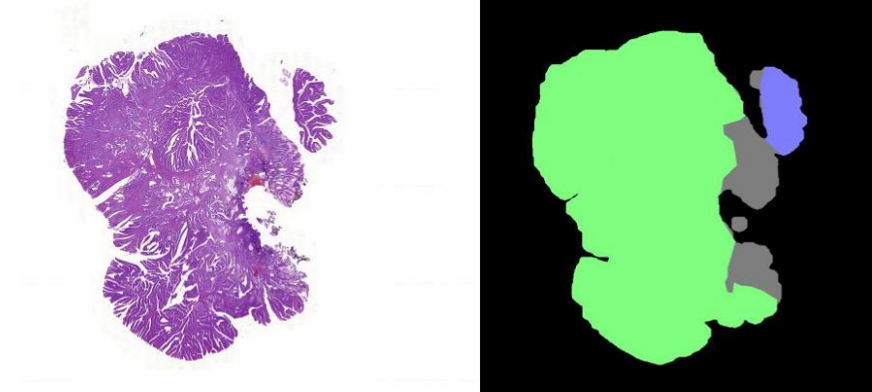
\includegraphics[width=0.70\textwidth]{img/mascara.png}
\end{center}
\captionof{figure}{Example WSI and its segmentation mask, with the annotated regions
color-coded (see Section~\ref{sec:anotacions-masques}).}
\label{fig-mask}

\subsection{Detailed \textit{Pipeline} Flow Diagram}
\label{app:pipeline-full}

\begin{figure}[H]
\centering
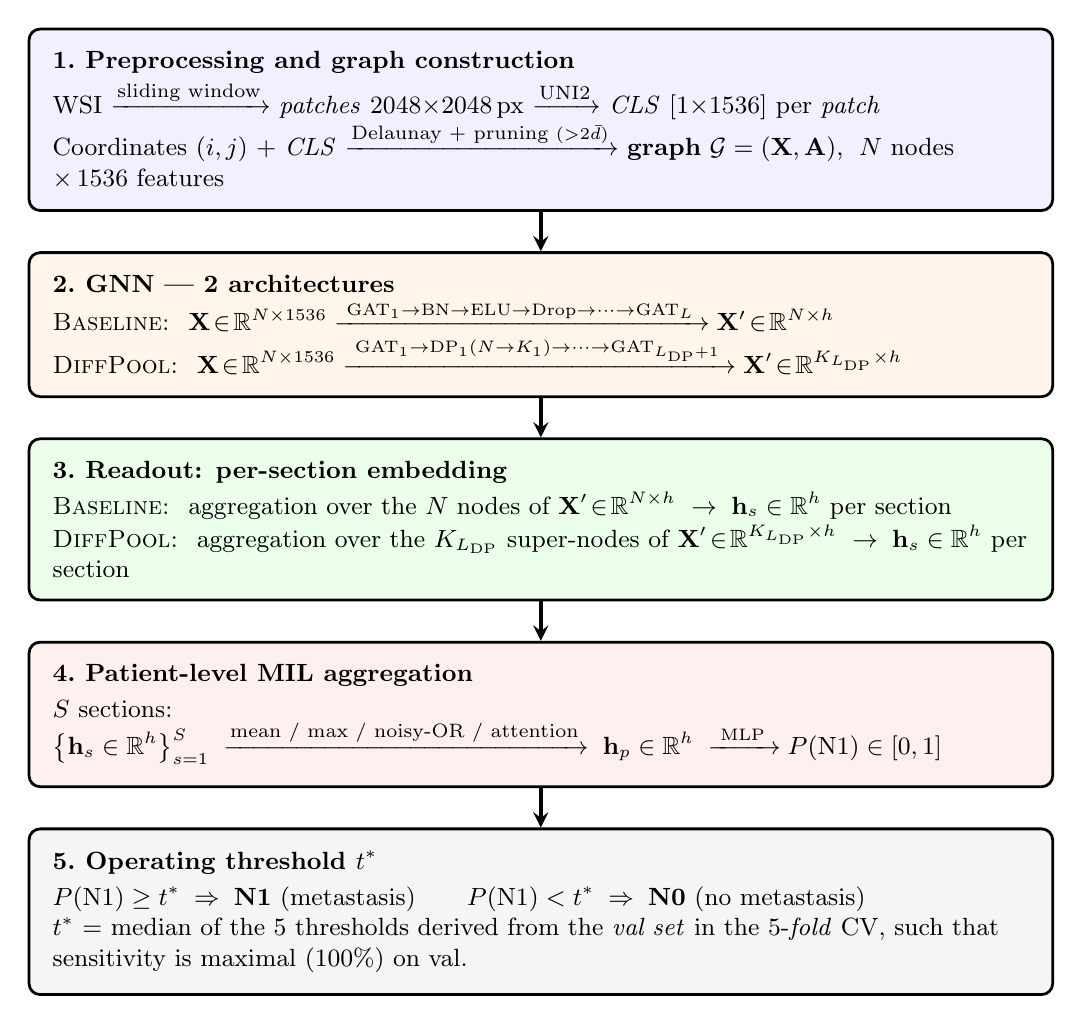
\begin{tikzpicture}[
    node distance=0.5cm,
    mainblock/.style={
        rectangle, rounded corners=4pt,
        draw=black, fill=blue!6, line width=1.0pt,
        minimum width=13cm, text width=12.4cm,
        inner sep=8pt, align=flush left, font=\small
    },
    arr/.style={->, >=stealth, line width=1.4pt, color=black},
]

\node[mainblock] (b1) {
  \textbf{1.\ Preprocessing and graph construction}\\[2pt]
  WSI $\xrightarrow{\text{\scriptsize sliding window}}$
  \textit{patches} $2048{\times}2048\,\text{px}$
  $\xrightarrow{\text{\scriptsize UNI2}}$ \textit{CLS} $[1{\times}1536]$ per \textit{patch}\\
  Coordinates $(i,j)$ + \textit{CLS}
  $\xrightarrow{\text{\scriptsize Delaunay + pruning }(>2\bar{d})}$
  \textbf{graph} $\mathcal{G}=(\mathbf{X},\mathbf{A})$,\; $N$ nodes $\times\,1536$ features
};

\node[mainblock, fill=orange!8, below=0.5cm of b1] (b2) {
  \textbf{2.\ GNN --- 2 architectures}\\[3pt]
  \textsc{Baseline:}\;
  $\mathbf{X}\!\in\!\mathbb{R}^{N\times 1536}
  \xrightarrow{\;\text{GAT}_1\to\text{BN}\to\text{ELU}\to\text{Drop}\to\cdots\to\text{GAT}_L\;}
  \mathbf{X}'\!\in\!\mathbb{R}^{N\times h}$\\[1pt]
  \textsc{DiffPool:}\;
  $\mathbf{X}\!\in\!\mathbb{R}^{N\times 1536}
  \xrightarrow{\;\text{GAT}_1\to\text{DP}_1(N\to K_1)\to\cdots\to\text{GAT}_{L_{\text{DP}}+1}\;}
  \mathbf{X}'\!\in\!\mathbb{R}^{K_{L_{\text{DP}}}\times h}$
};

\node[mainblock, fill=green!8, below=0.5cm of b2] (b3) {
  \textbf{3.\ Readout: per-section embedding}\\[2pt]
  \textsc{Baseline:}\;
  aggregation over the $N$ nodes of $\mathbf{X}'\!\in\!\mathbb{R}^{N\times h}$
  $\;\to\;\mathbf{h}_s \in \mathbb{R}^{h}$ per section\\[1pt]
  \textsc{DiffPool:}\;
  aggregation over the $K_{L_{\text{DP}}}$ super-nodes of $\mathbf{X}'\!\in\!\mathbb{R}^{K_{L_{\text{DP}}}\times h}$
  $\;\to\;\mathbf{h}_s \in \mathbb{R}^{h}$ per section
};

\node[mainblock, fill=red!6, below=0.5cm of b3] (b4) {
  \textbf{4.\ Patient-level MIL aggregation}\\[2pt]
  $S$ sections:\;
  $\bigl\{\mathbf{h}_s \in \mathbb{R}^{h}\bigr\}_{s=1}^{S}
  \;\xrightarrow{\text{\scriptsize mean / max / noisy-OR / attention}}\;
  \mathbf{h}_p \in \mathbb{R}^{h}
  \;\xrightarrow{\;\text{MLP}\;}
  P(\mathrm{N1}) \in [0,1]$
};

\node[mainblock, fill=gray!8, below=0.5cm of b4] (b5) {
  \textbf{5.\ Operating threshold $t^*$}\\[2pt]
  $P(\mathrm{N1}) \geq t^*\;\Rightarrow\;\mathbf{N1}$ (metastasis)\qquad
  $P(\mathrm{N1}) < t^*\;\Rightarrow\;\mathbf{N0}$ (no metastasis)\\
  $t^*$ = median of the 5 thresholds derived from the \textit{val set} in the 5-\textit{fold} CV,
  such that sensitivity is maximal (100\%) on val.
};

\foreach \a/\b in {b1/b2, b2/b3, b3/b4, b4/b5}
  \draw[arr] (\a.south) -- (\b.north);

\end{tikzpicture}
\caption{Flow diagram of the complete \textit{pipeline}, from the WSI to the N0/N1 decision. The five
blocks are described in Section~\ref{sec:pipeline-overview}.}
\label{fig:pipeline-full}
\end{figure}

\newpage

\subsection{Architecture Variants of the \textit{GATClassifier}}
\label{app:model-variants}

Diagram~\ref{fig:gat-variants} shows how the \textbf{same input graph}
can be processed in very different ways depending on the configuration: blue
boxes represent learned layers and dashed orange boxes the configurable
optimization axes.

\begin{figure}[H]
\centering
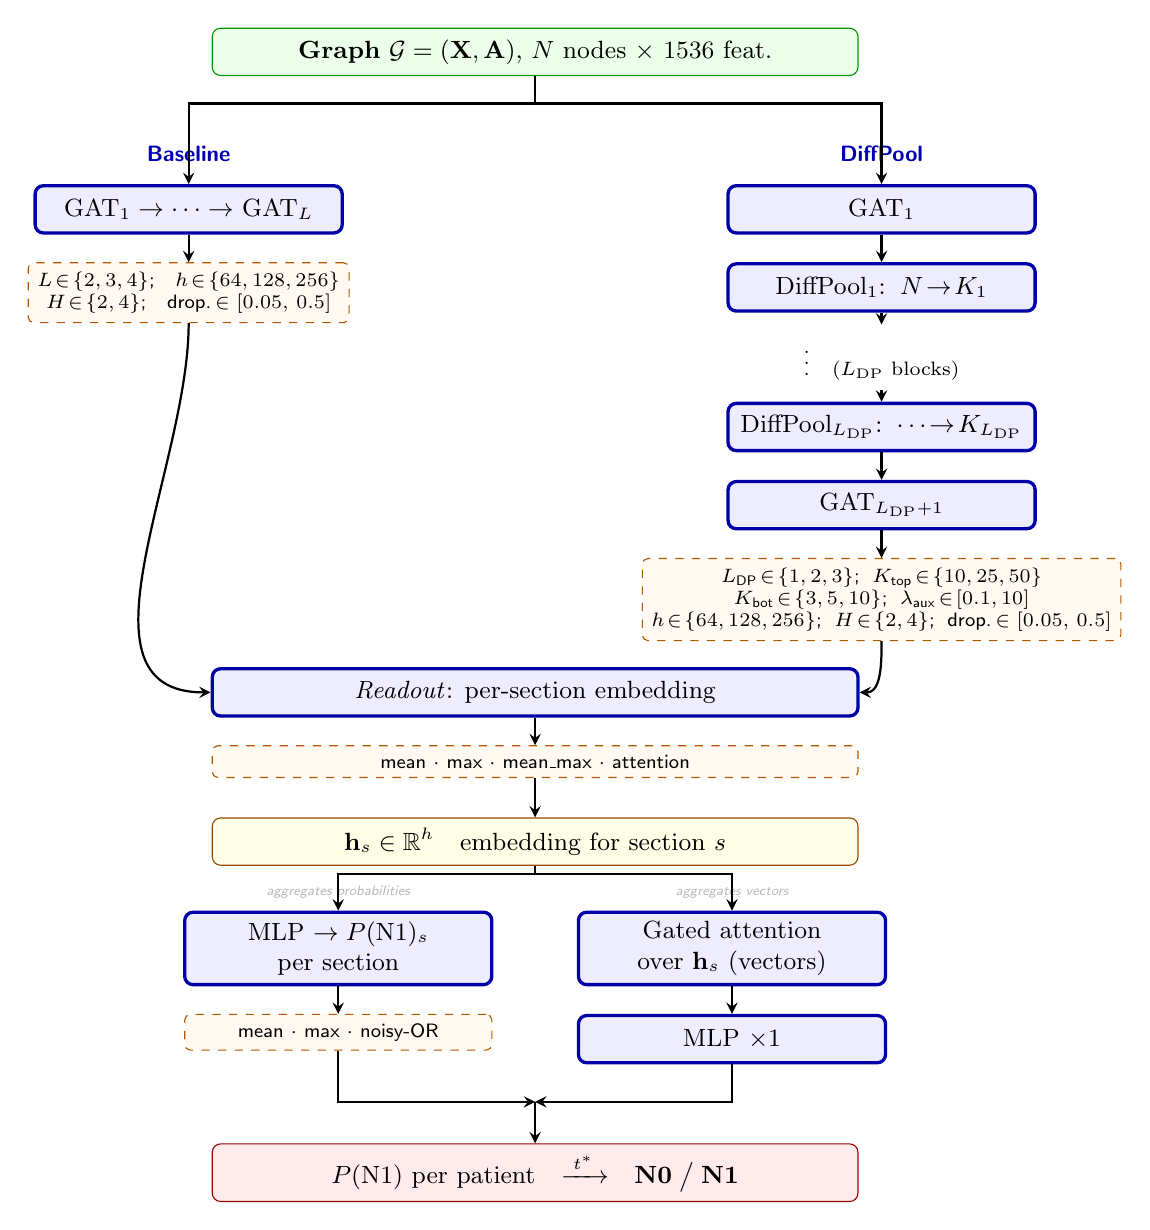
\begin{tikzpicture}[
    bblue/.style={rectangle, rounded corners=3pt,
                  draw=blue!65!black, line width=1.2pt, fill=blue!7,
                  minimum width=3.9cm, minimum height=0.6cm,
                  align=center, font=\small},
    opt/.style={rectangle, rounded corners=2pt,
                draw=orange!70!black, dashed, fill=orange!5,
                minimum width=3.9cm,
                align=center, font=\sffamily\scriptsize},
    inp/.style={rectangle, rounded corners=3pt,
                draw=green!60!black, fill=green!8,
                minimum width=8.2cm, minimum height=0.6cm,
                align=center, font=\small},
    mid/.style={rectangle, rounded corners=3pt,
                draw=orange!60!black, fill=yellow!10,
                minimum width=8.2cm, minimum height=0.6cm,
                align=center, font=\small},
    outbox/.style={rectangle, rounded corners=3pt,
                draw=red!60!black, fill=red!8,
                minimum width=8.2cm, minimum height=0.6cm,
                align=center, font=\small},
    arr/.style={->, >=stealth, thick},
]

%% ─── Input ──────────────────────────────────────────────────────────────────
\node[inp] (in) at (0,0)
    {\textbf{Graph} $\mathcal{G}=(\mathbf{X},\mathbf{A})$,
     $N$ nodes $\times$ 1536 feat.};

%% ─── BASELINE (left) ────────────────────────────────────────────────────────
\node[font=\small\bfseries\sffamily, text=blue!70!black]
     at (-4.4,-1.3) {\footnotesize\textsc{Baseline}};

\node[bblue] (b_gat) at (-4.4,-2.0)
    {GAT$_1 \to \cdots \to$ GAT$_L$};

\node[opt, below=0.35cm of b_gat] (b_gat_opt)
    {$L\!\in\!\{2,3,4\}$;\quad$h\!\in\!\{64,128,256\}$\\
     $H\!\in\!\{2,4\}$;\quad drop.$\,\in[0.05,\,0.5]$};

%% ─── DIFFPOOL (right) ───────────────────────────────────────────────────────
\node[font=\small\bfseries\sffamily, text=blue!70!black]
     at (4.4,-1.3) {\footnotesize\textsc{DiffPool}};

\node[bblue] (d_gat1) at (4.4,-2.0)
    {GAT$_1$};

\node[bblue, below=0.35cm of d_gat1] (d_dp1)
    {DiffPool$_1$:\;\;$N\!\to\!K_1$};

\node[font=\scriptsize, below=0.15cm of d_dp1] (d_vdots)
    {$\vdots$\quad($L_{\text{DP}}$ blocks)};

\node[bblue, below=0.15cm of d_vdots] (d_dpn)
    {DiffPool$_{L_{\text{DP}}}$:\;\;$\cdots\!\to\!K_{L_{\text{DP}}}$};

\node[bblue, below=0.35cm of d_dpn] (d_gatn)
    {GAT$_{L_{\text{DP}}+1}$};

\node[opt, below=0.35cm of d_gatn, minimum width=4.2cm] (d_dp_opt)
    {$L_{\text{DP}}\!\in\!\{1,2,3\}$;\;
     $K_{\text{top}}\!\in\!\{10,25,50\}$\\
     $K_{\text{bot}}\!\in\!\{3,5,10\}$;\;
     $\lambda_{\text{aux}}\!\in\![0.1,10]$\\
     $h\!\in\!\{64,128,256\}$;\;
     $H\!\in\!\{2,4\}$;\; drop.$\,\in[0.05,\,0.5]$};

%% ─── Readout unificat ────────────────────────────────────────────────────────
\coordinate (ro_y) at ($(d_dp_opt.south)+(0,-0.65)$);
\node[bblue, minimum width=8.2cm] (ro_block) at (0,0 |- ro_y)
    {\textit{Readout}: per-section embedding};
\node[opt, minimum width=8.2cm, below=0.35cm of ro_block] (ro_opt)
    {mean $\cdot$ max $\cdot$ mean\_max $\cdot$ attention};

%% ─── Embedding ───────────────────────────────────────────────────────────────
\node[mid, below=0.5cm of ro_opt] (emb)
    {$\mathbf{h}_s \in \mathbb{R}^{h}$\quad embedding for section $s$};

%% ─── Fork MIL: A = over probabilities / B = over vectors ──────────────────
\coordinate (emb_fk) at ($(emb.south)+(0,-1.05)$);

%% Branch A (x = −2.5): per-section MLP → aggregate scalar P(N1)
\node[bblue, minimum width=3.9cm] (mil_mlp) at (-2.5,0 |- emb_fk)
    {MLP $\to P(\text{N1})_s$\\per section};

\node[opt, minimum width=3.9cm, below=0.35cm of mil_mlp] (mil_scalar_opts)
    {mean $\cdot$ max $\cdot$ noisy-OR};

%% Branch B (x = +2.5): aggregate h_s vectors via attention → MLP once
\node[bblue, minimum width=3.9cm] (mil_att) at (2.5,0 |- emb_fk)
    {Gated attention\\over $\mathbf{h}_s$ (vectors)};

\node[bblue, minimum width=3.9cm, below=0.35cm of mil_att] (mil_att_mlp)
    {MLP $\times$1};

%% MIL branch labels
\node[font=\sffamily\tiny\itshape, text=gray!55,
      above=0.03cm of mil_mlp, anchor=south] {aggregates probabilities};
\node[font=\sffamily\tiny\itshape, text=gray!55,
      above=0.03cm of mil_att, anchor=south] {aggregates vectors};

%% ─── Output ─────────────────────────────────────────────────────────────────
\coordinate (conv_y) at ($(mil_scalar_opts.south)+(0,-0.65)$);
\coordinate (conv)   at (0,0 |- conv_y);
\node[outbox, minimum width=8.2cm] (outbox) at ($(conv)+(0,-0.9)$)
    {$P(\text{N1})$ per patient\quad
     $\xrightarrow{\;t^*\;}$\quad \textbf{N0}\;\big/\;\textbf{N1}};

%% ─── Fork from input ─────────────────────────────────────────────────────
\draw[arr] (in.south) -- ++(0,-0.35) -| (b_gat.north);
\draw[arr] (in.south) -- ++(0,-0.35) -| (d_gat1.north);

%% ─── Baseline ────────────────────────────────────────────────────────────────
\draw[arr] (b_gat) -- (b_gat_opt);

%% ─── DiffPool ────────────────────────────────────────────────────────────────
\draw[arr] (d_gat1)   -- (d_dp1);
\draw[arr] (d_dp1)    -- (d_vdots);
\draw[arr] (d_vdots)  -- (d_dpn);
\draw[arr] (d_dpn)    -- (d_gatn);
\draw[arr] (d_gatn)   -- (d_dp_opt);

%% ─── Convergence of architectures → unified readout ───────────────────────────
\draw[arr] (b_gat_opt.south) to[out=-90, in=180] (ro_block.west);
\draw[arr] (d_dp_opt.south)  to[out=-90, in=0]   (ro_block.east);
\draw[arr] (ro_block) -- (ro_opt);
\draw[arr] (ro_opt)   -- (emb);

%% ─── Fork MIL ────────────────────────────────────────────────────────────────
\draw[arr] (emb.south) -- ++(0,-0.1) -| (mil_mlp.north);
\draw[arr] (emb.south) -- ++(0,-0.1) -| (mil_att.north);
\draw[arr] (mil_mlp)   -- (mil_scalar_opts);
\draw[arr] (mil_att)   -- (mil_att_mlp);

%% ─── Convergence MIL → output ──────────────────────────────────────────────
\draw[arr] (mil_scalar_opts.south) |- (conv);
\draw[arr] (mil_att_mlp.south)     |- (conv);
\draw[arr] (conv) -- (outbox.north);

\end{tikzpicture}
\caption{Architecture variants of the \textit{GATClassifier}: the same graph $\mathcal{G}$ is
processed by two branches (\textsc{Baseline} or \textsc{DiffPool}) that converge into a
unified \textit{readout} ($\mathbf{h}_s \in \mathbb{R}^{h}$ per section) and then into
MIL aggregation (Section~\ref{sec:mil}).
Symbols: $L$ GAT layers; $h$ hidden dim.; $H$ attention heads;
$L_{\text{DP}}$ DiffPool blocks; $K_\ell$ super-nodes per level;
$\lambda_{\text{aux}}$ auxiliary loss weight; $t^*$ val-set threshold.}
\label{fig:gat-variants}
\end{figure}

\newpage

\subsection{Hyperparameter Importance per Architecture}
\label{app:main-effects}

Table~\ref{tab:main-effects} shows the \textbf{fANOVA importance} of each optimization
axis, computed independently for each Optuna study (Baseline and
DiffPool).

\textbf{What is analyzed.} The analyzed variable is each \textit{trial}'s cross-validation objective
($\overline{\text{spec}}_{\text{CV}} - 10\cdot\max(0,
1-\overline{\text{sens}}_{\text{CV}})$, what the \textit{sweep} maximizes). The
\textit{functional ANOVA} fits a surrogate model (\textit{random forest}) over all
\textit{trials} and decomposes this objective's variance into each axis's contribution. The
reported importance is the fraction of variance explained by the axis alone (main
effect, in $[0, 1]$): the higher it is, the more that hyperparameter weighs on performance. They do not
sum to $1$ because interactions are not included. Axes specific to one branch
appear empty in the other column.

\begin{table}[H]
\centering
\caption{fANOVA importance per architecture. Empty cells indicate the axis does not apply to that branch.}
\label{tab:main-effects}
\small
\begin{tabular}{lcc}
\toprule
\textbf{Axis} & \textbf{Baseline} & \textbf{DiffPool} \\
\midrule
\multicolumn{3}{l}{\textit{Architecture-specific axes}} \\[2pt]
$L$ (GAT layers)                          & $0.017$ & --- \\
$L_{\text{DP}}$ (DiffPool blocks)         & --- & $0.062$ \\
$K_{\text{top}}$                          & --- & $0.027$ \\
$K_{\text{bot}}$                          & --- & $0.021$ \\
$\lambda_{\text{aux}}$                    & --- & $\mathbf{0.141}$ \\
\midrule
\multicolumn{3}{l}{\textit{Shared axes (optimized independently per study)}} \\[2pt]
\textit{Readout} (graph read-out)         & $0.079$ & $0.053$ \\
$h$ (hidden dim.)                         & $0.012$ & $0.027$ \\
$H$ (attention heads)                     & $0.024$ & $0.066$ \\
\textit{Dropout}                          & $0.054$ & $0.079$ \\
MIL aggregation                           & $\mathbf{0.640}$ & $\mathbf{0.224}$ \\
$\eta$ (\textit{learning rate})           & $0.036$ & $\mathbf{0.129}$ \\
$\lambda_{\text{wd}}$ (\textit{weight decay}) & $0.020$ & $0.083$ \\
$w_+$ (\textit{pos\_weight})              & $0.075$ & $0.046$ \\
\textit{Optimizer}                        & $0.005$ & $0.015$ \\
\textit{Scheduler}                        & $0.019$ & $0.008$ \\
\textit{Grad clipping}                    & $0.017$ & $0.019$ \\
\bottomrule
\end{tabular}
\end{table}

\subsection{Hyperparameters of the Selected Model and Best DiffPool}
\label{app:best-params}

Table~\ref{tab:best-params} summarizes the configuration of the GAT Baseline and GAT+DiffPool,
already evaluated per the procedure in Table~\ref{tab:configs-compare}.

\begin{table}[H]
\centering
\caption{Configuration of the GAT Baseline and GAT+DiffPool.}
\label{tab:best-params}
\small
\begin{tabular}{lcc}
\toprule
\textbf{Axis} & \textbf{Baseline} & \textbf{DiffPool} \\
\midrule
\multicolumn{3}{l}{\textit{Architecture --- Baseline}} \\[2pt]
$L$ (GAT layers)                          & $3$                      & --- \\
$h$ / $H$ / \textit{Dropout}             & $256$ / $4$ / $0.3$    & --- \\
\textit{Readout}                         & \textit{attention}       & --- \\
\midrule
\multicolumn{3}{l}{\textit{Architecture --- DiffPool}} \\[2pt]
$L$ (= $L_{\text{DP}}+1$)               & ---                      & $3$ \\
$L_{\text{DP}}$ / $K_{\text{top}},K_{\text{bot}}$ & ---           & $2$ / $50,\,3$ \\
$h$ / $H$ / \textit{Dropout}             & ---                      & $128$ / $2$ / $0.437$ \\
$\lambda_{\text{aux}}$                   & ---                      & $0.108$ \\
\textit{Readout}                         & ---                      & \textit{mean\_max} \\
\midrule
\multicolumn{3}{l}{\textit{Training and regularization}} \\[2pt]
MIL                                      & \textit{mean}            & \textit{mean} \\
$\eta$ / $\lambda_{\text{wd}}$ / $w_+$   & $3\!\cdot\!10^{-4}$ / $10^{-4}$ / $2.0$ & $5.3\!\cdot\!10^{-4}$ / $5.5\!\cdot\!10^{-3}$ / $3.52$ \\
\textit{Optimizer} / \textit{Scheduler}  & \textit{adam} / \textit{plateau} & \textit{adam} / \textit{cosine} \\
\midrule
\multicolumn{3}{l}{\textit{Metrics re-evaluated on the test set}} \\[2pt]
AUC CV ($\pm$std)                        & $0.862\!\pm\!0.038$  & $0.847\!\pm\!0.048$ \\
AUC test                                 & $\mathbf{0.875}$       & $0.786$ \\
Sens.\ / Spec.\ test @$t^*$              & $\mathbf{1.000\,/\,0.575}$ & $0.625\,/\,0.700$ \\
$t^*$                                    & $0.133$                & $0.303$ \\
\bottomrule
\end{tabular}
\end{table}

% \newpage
%
% \subsection{Confusion Matrix and $P(\mathrm{N1})$ Distribution}
% \label{app:prob-dist}
%
% Table~\ref{tab:cm} shows the confusion matrix of the selected model on the test set
% ($n\!=\!56$, $t^*\!=\!0.133$): PPV $=0.485$, NPV $=1.000$.
%
% \begin{table}[H]
% \centering
% \caption{Confusion matrix of the selected GAT Baseline on the test set ($n\!=\!56$, $t^*\!=\!0.133$).}
% \label{tab:cm}
% \small
% \begin{tabular}{llcc}
% \toprule
%  & & \multicolumn{2}{c}{\textbf{Actual diagnosis}} \\
%  & & \textbf{N0} & \textbf{N1} \\
% \midrule
% \multirow{2}{*}{\textbf{Prediction}}
%   & \textbf{N0} & 23 & 0 \\
%   & \textbf{N1} & 17 & 16 \\
% \bottomrule
% \end{tabular}
% \end{table}
%
% Figure~\ref{fig:prob-dist} shows the $P(\mathrm{N1})$ distribution for each
% test patient, split by true label. All 16 N1 cases fall to the right of
% $t^*\!=\!0.133$; of the 40 N0 cases, 23 fall to the left.
%
% \begin{figure}[H]
%     \centering
%     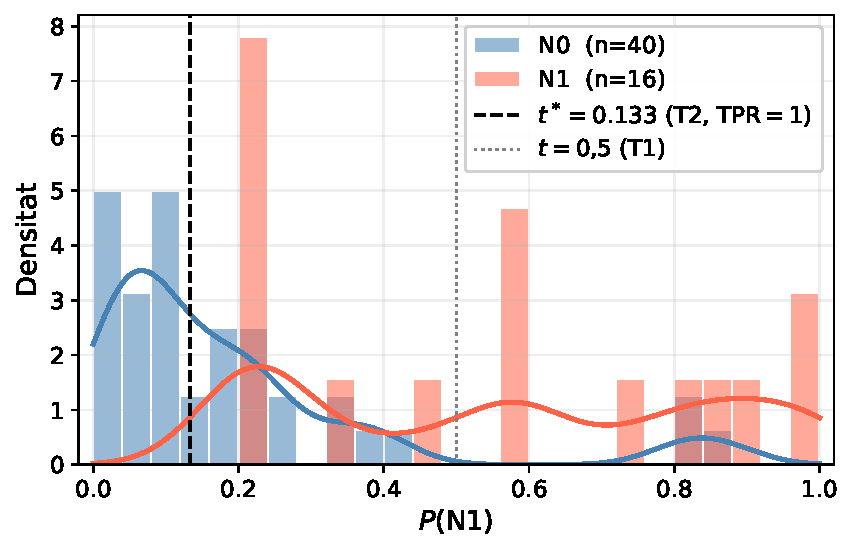
\includegraphics[width=0.75\textwidth]{img/prob_dist.pdf}
%     \caption{$P(\mathrm{N1})$ distribution on the test set ($n\!=\!56$)
%     for the selected GAT Baseline. Blue: N0 ($n\!=\!40$);
%     red: N1 ($n\!=\!16$). Dashed line: $t^*\!=\!0.133$ (T2, TPR$=1$);
%     dotted line: $t\!=\!0.5$ (T1). All N1 cases fall to the right of $t^*$.}
%     \label{fig:prob-dist}
% \end{figure}
%
\newpage

\subsection{Bayesian Search Space}
\label{app:sweep-config}

Table~\ref{tab:sweep-config} lists the optimization axes, their ranges, and the architecture
branch to which they apply. The search is done with \textit{TPE} (Optuna); each \textit{trial} evaluates
a configuration with 5-\textit{fold} CV over the train+val \textit{pool}. The two architectures
are optimized in \textbf{isolated Optuna studies} (separate SQLite databases): axes specific to each
architecture are not mixed, and shared axes are optimized independently for each branch.

\begin{table}[H]
\centering
\caption{Bayesian \textit{sweep} axes (two isolated Optuna studies, one per architecture).}
\label{tab:sweep-config}
\small
\renewcommand{\arraystretch}{1.05}
\begin{tabular}{p{5.0cm}>{\raggedleft\arraybackslash}p{5.3cm}>{\raggedleft\arraybackslash}p{3.0cm}}
\toprule
\textbf{Axis} & \textbf{Values / range} & \textbf{Sampling type} \\
\midrule
\multicolumn{3}{l}{\textit{Model architecture --- Baseline}} \\[2pt]
$L$ (GAT layers)                             & 2, 3, 4                                    & integer \\
\textit{Readout}                            & mean, max, mean\_max, attention            & categorical \\
$h$ (hidden dimension)                       & 64, 128, 256                               & categorical \\
$H$ (attention heads)                        & 2, 4                                       & categorical \\
\textit{Dropout}                            & $[0.05,\,0.5]$                         & uniform \\
\midrule
\multicolumn{3}{l}{\textit{Model architecture --- DiffPool}} \\[2pt]
$L_{\text{DP}}$ (DiffPool blocks)            & 1, 2, 3                                    & integer \\
$K_{\text{top}}$ (1st-level super-nodes)    & 10, 25, 50                                 & categorical \\
$K_{\text{bot}}$ (last-level super-nodes) & 3, 5, 10                                   & categorical \\
\multicolumn{3}{l}{\quad\footnotesize(Intermediate: $K = \lfloor\sqrt{K_{\text{top}} \cdot K_{\text{bot}}}\rfloor$; clamp $K_{\text{bot}} < K_{\text{top}}$)} \\[2pt]
$\lambda_{\text{aux}}$ (aux.\ weight)           & $[0.1,\,10]$                             & log-uniform \\
\textit{Readout}                            & mean, max, mean\_max, attention            & categorical \\
$h$ (hidden dimension)                       & 64, 128, 256                               & categorical \\
$H$ (attention heads)                        & 2, 4                                       & categorical \\
\textit{Dropout}                            & $[0.05,\,0.5]$                         & uniform \\
\midrule
\multicolumn{3}{l}{\textit{MIL aggregation --- both architectures (optimized independently)}} \\[2pt]
MIL aggregation                               & mean, max, noisy-OR, attention             & categorical \\
\midrule
\multicolumn{3}{l}{\textit{Optimizer and regularization --- both (independently)}} \\[2pt]
\textit{Optimizer}                          & Adam, AdamW                                & categorical \\
\textit{Scheduler}                          & ReduceLROnPlateau, CosineAnnealingLR       & categorical \\
Learning rate                           & $[5\cdot10^{-5},\,5\cdot10^{-3}]$         & log-uniform \\
\textit{Weight decay}                       & $[10^{-5},\,10^{-2}]$                      & log-uniform \\
\textit{Grad.\ clipping}                     & 0, 1, 5                                    & categorical \\
N1 class weight ($w_+$)                       & $[1.5,\,8.0]$                          & uniform \\
\bottomrule
\end{tabular}
\end{table}

\textbf{Sweep objective:}
$\text{objective} = \overline{\text{spec}}_{\text{CV}} - 10 \cdot \max(0,\; 1 - \overline{\text{sens}}_{\text{CV}})$,
where $\overline{\text{spec}}_{\text{CV}}$ and $\overline{\text{sens}}_{\text{CV}}$ are the means
over the 5 \textit{val sets}, computed with the threshold $t^*$ derived from each \textit{fold}
(highest threshold with TPR$=1$). This is the \textbf{only} metric the TPE sees to decide
the next \textit{trial}'s parameters. The $\times 10$ penalty makes the TPE prioritize
$100\%$ sensitivity; any loss of sensitivity must be offset
by a much larger specificity gain (10 points for every point of sensitivity lost).

\subsection{Confusion Matrix of the Selected Model}
\label{app:cm}

Table~\ref{tab:cm} shows the confusion matrix of the selected GAT Baseline on the test set
($n\!=\!56$, $t^*\!=\!0.133$): all 16 N1 cases are detected (FN$=0$, NPV$=1.000$), and of the
40 N0 cases, 23 are classified correctly (17 FP, PPV$=0.485$).

\begin{table}[H]
\centering
\caption{Confusion matrix of the selected GAT Baseline on the test set ($n\!=\!56$, $t^*\!=\!0.133$).}
\label{tab:cm}
\small
\begin{tabular}{llcc}
\toprule
 & & \multicolumn{2}{c}{\textbf{Actual diagnosis}} \\
 & & \textbf{N0} & \textbf{N1} \\
\midrule
\multirow{2}{*}{\textbf{Prediction}}
  & \textbf{N0} & 23 & 0 \\
  & \textbf{N1} & 17 & 16 \\
\bottomrule
\end{tabular}
\end{table}

\end{document}
